\lhead{Capítulo 1}
\rhead{Dinámica Enerética en Modelos N-Body: Análisis de la Influencia de la Desviación Estándar en las Interacciones Partícula-vida}
\cfoot{\thepage}
\renewcommand{\headrulewidth}{1pt}
\renewcommand{\footrulewidth}{1pt}
\chapter{Análisis de la Influencia de la Desviación Estándar en las Interacciones Partícula-vida}

\section{Introducción}
En el enfoque de los sistemas N-body en la física computacional, el estudio de entidades interactivas adquiere un significado particular. El presente proyecto se inserta en este contexto, centrándose en el desentrañamiento de cómo la variabilidad en las fuerzas de interacción entre partículas, estratificadas a través de diferentes niveles de desviación estándar, influye en la energía global de un modelo abstracto denominado "partícula-vida". Inspirado por la importancia de comprender la dinámica intrincada de sistemas como los fluidos moleculares, estrellas enanas enanas blancas, o incluso agrupaciones galácticas, este estudio se propone analizar detalladamente cómo la incertidumbre inherente a estas interacciones puede dar lugar a patrones energéticos inesperados.

El término "partícula-vida" evoca la idea de un sistema que, aunque simplificado, captura elementos dinámicos vitalistas, donde cada partícula no solo sigue reglas físicas básicas sino que, bajo condiciones específicas, sus interacciones complejas dan lugar a fenómenos emergentes. A través de simulaciones avanzadas, este proyecto busca desvelar cómo la variabilidad en las fuerzas que gobiernan estas interacciones –modeladas mediante desviaciones estándar variable– puede generar cambios significativos en el comportamiento energético del sistema, lo que a su vez puede tener implicaciones en la comprensión de fenómenos físicos y biológicos.

\section{Título}
Dinámica y Energética del "Partícula-Vida": Análisis de la Desviación Estándar en las Interacciones

\section{Tema de Investigación}

Este proyecto aborda la simulación de un sistema compuesto por cuatro grupos de partículas con interacciones atractivas-repulsivas modeladas. Se investiga cómo la variabilidad en las fuerzas de interacción, expresada a través de diferentes niveles de desviación estándar, afecta la energía cinética y potencial del sistema. El objetivo es comprender cómo estas variaciones microscópicas pueden generar macroefectos significativos, utilizando técnicas de computación numérica avanzadas.

\section{Objetivos}

\subsection{Objetivo General}
Explorar la relación entre la desviación estándar en las fuerzas de interacción entre partículas y la energía total de un sistema multi-partícula, mediante simulaciones computacionales.

\subsection{Objetivos Específicos}
\begin{enumerate}
\item Implementar un modelo numérico que simule interacciones entre partículas basado en fuerzas que varían con la desviación estándar.
\item Evaluar la energía cinética y potencial del sistema para una serie de desviaciones estándar.
\item Graficar y analizar cómo la energía total del sistema cambia en respuesta a diferentes niveles de variabilidad en las interacciones.
\end{enumerate}

\section{Hipótesis de Investigación}
Aumentar la desviación estándar en las fuerzas de interacción entre partículas llevará a un aumento en la energía total del sistema, debido a una mayor actividad y variabilidad en las colisiones y movimientos.

\section{Justificación}
Este estudio es relevante porque brinda una visión computacional de cómo la incertidumbre en las fuerzas interatómicas puede influir en propiedades globales de un sistema, lo cual es fundamental en campos como la física de materiales, biología molecular y la simulación de fluidos complejos.

\section{Fundamentación Teórica}
La teoría detrás de este proyecto se basa en la física clásica de partículas, específicamente en las fuerzas de interacción newtonianas modificadas para incorporar una componente estocástica. Se utilizan conceptos de mecánica clásica y métodos numéricos para estimar y analizar la energía cinética y potencial.

\begin{itemize}
\item \textbf{Modelos Matemáticos y Algorítmicos}: Se emplearán modelos matemáticos para describir las fuerzas entre partículas y algoritmos numéricos para la simulación de su dinámica. Los modelos se basarán en las leyes de Newton con modificaciones estocásticas para incluir variabilidad en las fuerzas de interacción.
\item \textbf{Variables y Datos}: Las variables a utilizar incluyen posiciones, velocidades y fuerzas entre partículas y los parámetros que definen las fuerzas de interacción.
\item \textbf{Referencias Teóricas}: Las teorías y métodos utilizados se fundamentan en la mecánica clásica y la estadística, con énfasis en la simulación de sistemas dinámicos.

\section{Modelo Computacional y Algoritmo}

El modelo implementado utiliza NumPy y Numba para optimizar cálculos, mientras que Matplotlib se emplea para visualización. Se crean partículas con posiciones y velocidades iniciales, y se actualiza su energía y posición en función de fuerzas calculadas con una desviación estándar variable.

\subsection{Parámetros del Modelo}
Las variables independientes incluyen:
\begin{itemize}
\item \textbf{Número de Partículas}: Cuatro grupos de partículas, cada uno con un número configurable de partículas.
\item \textbf{Rango de Interacción}: Distancia máxima a la cual las fuerzas de interacción son significativas.
\item \textbf{Desviación Estándar de las Fuerzas}: Rango de valores para la desviación estándar de las fuerzas de interacción.
\end{itemize}

\subsection{Parámetros de los Métodos Computacionales}
Para la integración de las ecuaciones de movimiento, se utilizará el método de Verlet con un paso temporal (\texttt{dt}) ajustable para garantizar la estabilidad numérica.

\subsection{Inicialización de Partículas}
Las partículas se distribuyen aleatoriamente en una ventana de visualización.

\subsection{Actualización de Posiciones}
La función \texttt{update_positions} se encarga de actualizar las posiciones de las partículas en función de las fuerzas calculadas y las condiciones de frontera del sistema.

\begin{lstlisting}[language=Python]
    @njit(fastmath=True)
    def update_positions(atoms_np, forces, dt, window_width, window_height):
        for i, atom in enumerate(atoms_np):
            atom[:2] += forces[i] * dt
            if atom[0] < 0:
                atom[0] = 0
                atom[2] *= -1
            elif atom[0] > window_width:
                atom[0] = window_width
                atom[2] *= -1
            if atom[1] < 0:
                atom[1] = 0
                atom[3] *= -1
            elif atom[1] > window_height:
                atom[1] = window_height
                atom[3] *= -1
\end{lstlisting}

\subsection{Definición de las interacciones entre partículas}
Las interacciones entre partículas se definen a través de un arreglo de interacciones que varía con la desviación estándar. Uno de los hallazgos clave de esta simulación es la normalización de norma L2 de las interacciones para garantizar una escala adecuada. Cuando no se normalizan, las interacciones pueden volverse estables con mucha rapidez, lo que limita la variabilidad en el sistema o volverse demasiado inestables con rapidez transformando el sistema en solo ruido blanco sin patrones.

\begin{lstlisting}[language=Python]  
# Crear una lista de interacciones con desviación estándar variable
lista_interacciones = np.random.normal(0, 1.25, 16)   
# Normalizar las interacciones
lista_interacciones = np.array(lista_interacciones) / np.linalg.norm(lista_interacciones)
\end{lstlisting}

\subsection{Realizaciones}
Para obtener resultados estadísticamente significativos, se realizarán múltiples simulaciones con diferentes configuraciones de desviación estándar, y se promediarán los resultados para cada nivel de variabilidad. Se presentarán gráficos que muestren la evolución de la energía total del sistema en función de la desviación estándar, lo que permitirá analizar cómo la variabilidad en las fuerzas de interacción afecta la energía del sistema.

\subsection{Cálculos Matemáticos}
Los cálculos matemáticos se basan en la mecánica clásica y las leyes de Newton, con modificaciones estocásticas para incorporar variabilidad en las fuerzas de interacción. Para definir las interacciones entre partículas, se utilizan un muestreo aleatorio de la distribución normal con media 0 para recibir valores positivos y negativos, y se normalizan para garantizar una escala adecuada variando solo la desviación estándar.
\subsection{Resultados}
Los resultados se presentarán en forma de gráficos que muestren la evolución de la energía total del sistema en función de la desviación estándar. Se asegurará una presentación estética adecuada, con un tamaño de letra, número, tipografía y calidad adecuados.

\section{Optimización y Desafíos}

Durante la implementación del modelo, se encontró que el procesamiento de grandes cantidades de partículas planteaba un reto significativo en términos de rendimiento. Inicialmente, la versión sin optimizar del código, basado en conceptos similares a aquellos descritos en [Referencia GitHub, año], no soportaba satisfactoriamente más de 200 partículas por grupo debido a limitaciones computacionales. Para superar este obstáculo, se recurrió a la utilización intensiva de Numba, un compilador Just-In-Time (JIT) para Python y NumPy, que permitió un aumento notable en la velocidad de cálculo.

La función \texttt{calculate_forces}, por ejemplo, fue crucial para este proceso de optimización, garantizando que las interacciones entre miles de partículas pudieran ser calculadas eficientemente.

\begin{lstlisting}[language=Python]
    @njit(fastmath=True)
    def calculate_forces(atoms1_np, atoms2_np, g):
        forces = np.zeros_like(atoms1_np[:, :2])
        for i, a in enumerate(atoms1_np):
            ax, ay = a[:2]
            for b in atoms2_np:
                bx, by = b[:2]
                dx, dy = ax - bx, ay - by
                d = np.sqrt(dx**2 + dy**2)
                if 0 < d < 80:
                    F = (g * 1) / d
                    fx, fy = F * dx, F * dy
                    forces[i, 0] += fx
                    forces[i, 1] += fy
        return forces
\end{lstlisting}

Esta estrategia permitió aumentar la cantidad de partículas simuladas por grupo a 2000, sin comprometer el tiempo de ejecución ni la legibilidad del código. Además, la gestión cuidadosa de las condiciones de frontera y la elección adecuada de parámetros como el paso temporal (\texttt{dt}) fueron fundamentales para mantener la precisión y la estabilidad numérica del modelo.

\section{Resultados y Discusión}

En esta sección, se analizan los resultados obtenidos mediante la simulación del comportamiento energético de un sistema compuesto por partículas interactivas bajo diferentes niveles de variabilidad en sus fuerzas de interacción.

\subsection{Simulación del Sistema}

El código desarrollado inicia creando cuatro grupos de partículas (amarillas, rojas, verdes y azules), cada uno con 2000 partículas, distribuidas aleatoriamente dentro de una ventana de 800x800 píxeles. A través de funciones optimizadas con Numba, se calculan las fuerzas entre partículas considerando una fuerza que disminuye con la distancia, con una modulación basada en una matriz de interacciones que varía según una desviación estándar dada. Este proceso, iterado a lo largo de 1000 pasos de tiempo, permite calcular la energía cinética y potencial acumulada, lo que conduce a un valor promedio de energía para cada nivel de desviación estándar.

\subsection{Análisis de Energía vs. Desviación Estándar}

\begin{figure}[ht!]
\centering
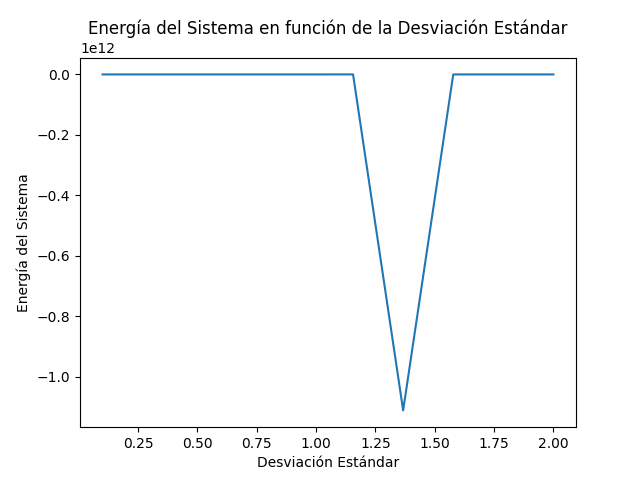
\includegraphics[width=0.8\linewidth]{./mnt/data/desviacion.png}
\caption{Evolución de la energía promedio del sistema en función de la desviación estándar de las fuerzas de interacción.}
\label{fig
}
\end{figure}

La figura \ref{fig
} muestra cómo la energía promedio del sistema varía con diferentes desviaciones estándar. Nótese cómo la energía total del sistema se mantiene constante en 0 para desviaciones estándar bajas y altas, pero experimenta una caída significativa alrededor de una desviación estándar de 1.25. Este comportamiento indica que, bajo ciertas condiciones de variabilidad en las fuerzas de interacción, la energía del sistema crece hacia lo negativo de manera abrupta, lo que sugiere una mayor movimiento e interacción entre las partículas.
\subsection{Discusión}

En esta reflexión, se destaca cómo el análisis detallado de los resultados revela un patrón complejo en la relación entre la variabilidad en las fuerzas de interacción y la energía total del sistema. La observación de una relación no lineal sugiere un punto crítico en la desviación estándar, donde el sistema experimenta cambios drásticos en su comportamiento energético. Este efecto demuestra que la aleatoriedad, aunque puede generar configuraciones menos predecibles, bajo ciertas condiciones, puede también conducir a estados más ordenados y de menor energía, un fenómeno que desafía intuiciones simples y pone de manifiesto la riqueza de los sistemas complejos.

La importancia de la normalización en la distribución de las fuerzas de interacción se pone en evidencia a través de tus experimentos repetidos. Al encontrar que una desviación estándar excesivamente alta oblitera los patrones y las interacciones significativas entre las partículas, mientras que un valor demasiado bajo lleva a una rápida estabilización, se resalta la delicada equilibrio entre aleatoriedad y estructura en sistemas dinámicos. Esta sensibilidad a las condiciones iniciales y a la parametrización es fundamental en la comprensión de fenómenos emergentes en física y química, desde la formación de estructuras moleculares hasta la dinámica de fluidos complejos.

Además, esta investigación sugiere la necesidad de un enfoque cuidadoso en la selección de parámetros en modelos computacionales, ya que incluso pequeñas variaciones pueden tener impactos significativos en los resultados finales. Este trabajo contribuye a la comprensión de cómo la complejidad surge de las interacciones básicas, iluminando áreas donde la teoría y la simulación deben trabajar juntas para desentrañar los mecanismos subyacentes a los procesos macroscópicos a través del análisis de las dinámicas microscópicas.

En términos de aplicaciones, estos hallazgos podrían ser cruciales en la modelación de sistemas biológicos, donde la variabilidad en las interacciones moleculares es fundamental para procesos como la formación de proteínas o la propagación de señales celulares. También tienen implicaciones en la ingeniería de materiales, donde el control preciso de las interacciones a nivel atómico o molecular puede conducir a propiedades materialmente deseadas.

En conclusión, este estudio destaca la relevancia de entender y controlar la aleatoriedad en las interacciones partícula-partícula, ofreciendo una ventana valiosa hacia los mecanismos que rigen la energía y la estabilidad en sistemas complejos. La combinación de experimentación computacional y análisis riguroso brinda una herramienta poderosa para explorar y predecir comportamientos emergentes en sistemas físicos y biológicos, allanando el camino para futuras investigaciones interdisciplinarias en la frontera de la física, la química y la biología.